% 
% Annual Cognitive Science Conference
% Sample LaTeX Paper -- Proceedings Format
% 

% Original : Ashwin Ram (ashwin@cc.gatech.edu)       04/01/1994
% Modified : Johanna Moore (jmoore@cs.pitt.edu)      03/17/1995
% Modified : David Noelle (noelle@ucsd.edu)          03/15/1996
% Modified : Pat Langley (langley@cs.stanford.edu)   01/26/1997
% Latex2e corrections by Ramin Charles Nakisa        01/28/1997 
% Modified : Tina Eliassi-Rad (eliassi@cs.wisc.edu)  01/31/1998
% Modified : Trisha Yannuzzi (trisha@ircs.upenn.edu) 12/28/1999 (in process)
% Modified : Mary Ellen Foster (M.E.Foster@ed.ac.uk) 12/11/2000
% Modified : Ken Forbus                              01/23/2004
% Modified : Eli M. Silk (esilk@pitt.edu)            05/24/2005
% Modified : Niels Taatgen (taatgen@cmu.edu)         10/24/2006
% Modified : David Noelle (dnoelle@ucmerced.edu)     11/19/2014


%% Change "letterpaper" in the following line to "a4paper" if you must.

\documentclass[10pt,letterpaper]{article}

\usepackage{cogsci}
\usepackage{comment}
\usepackage{pslatex}
\usepackage{apacite}
\usepackage{amsmath,amssymb}
\usepackage{graphicx}
\usepackage{subcaption}
\usepackage{color}
\usepackage{url}
\usepackage{todonotes}
\usepackage{mathtools}
\usepackage{stmaryrd}
\usepackage{booktabs}
\usepackage{array}
\usepackage{caption}
\usepackage{sidecap}
\usepackage{capt-of}
\usepackage{nicefrac}
\usepackage[export]{adjustbox}
\usepackage{makecell}
\hyphenpenalty=100
\renewcommand\theadfont{\normalsize}
\usepackage[font={footnotesize}]{caption}
\newcommand{\jefan}[1]{{\color{blue}{[jefan: #1]}}}
\newcommand{\kushin}[1]{{\color{orange}{[kushin: #1]}}}
\newcommand\norm[1]{\left\lVert#1\right\rVert}


\title{Communicating semantic part information in drawings}

% \author{\begin{tabular}[htbp]{c@{\extracolsep{1em}}c@{\extracolsep{1em}}c@{\extracolsep{1em}}c} \\
% {\large \bf Kushin Mukherjee} & {\large \bf Robert X. D. Hawkins} & {\large \bf Judith E. Fan}\\
% Department of Cognitive Science  & Department of Psychology & Department of Psychology \\ 
% Vassar College & Stanford University & Stanford University \\
% \texttt{kumukherjee@vassar.edu} & \texttt{rxdh@stanford.edu} & \texttt{jefan@stanford.edu} \\
% \end{tabular}
% }

\author{{\large \bf Kushin Mukherjee\textsuperscript{1}, Robert X. D. Hawkins\textsuperscript{2}, Judith E. Fan\textsuperscript{2,3}} \\
\textsuperscript{1}Department of Cognitive Science, Vassar College, \\
\textsuperscript{2}Department of Psychology, Stanford University, \\
\textsuperscript{3}Department of Psychology, University of California, San Diego}

%\author{\large \bf Anonymous CogSci submission}

\begin{document}
\makeatletter
\let\@oldmaketitle\@maketitle% Store \@maketitle
\renewcommand{\@maketitle}{\@oldmaketitle% Update \@maketitle to insert...
  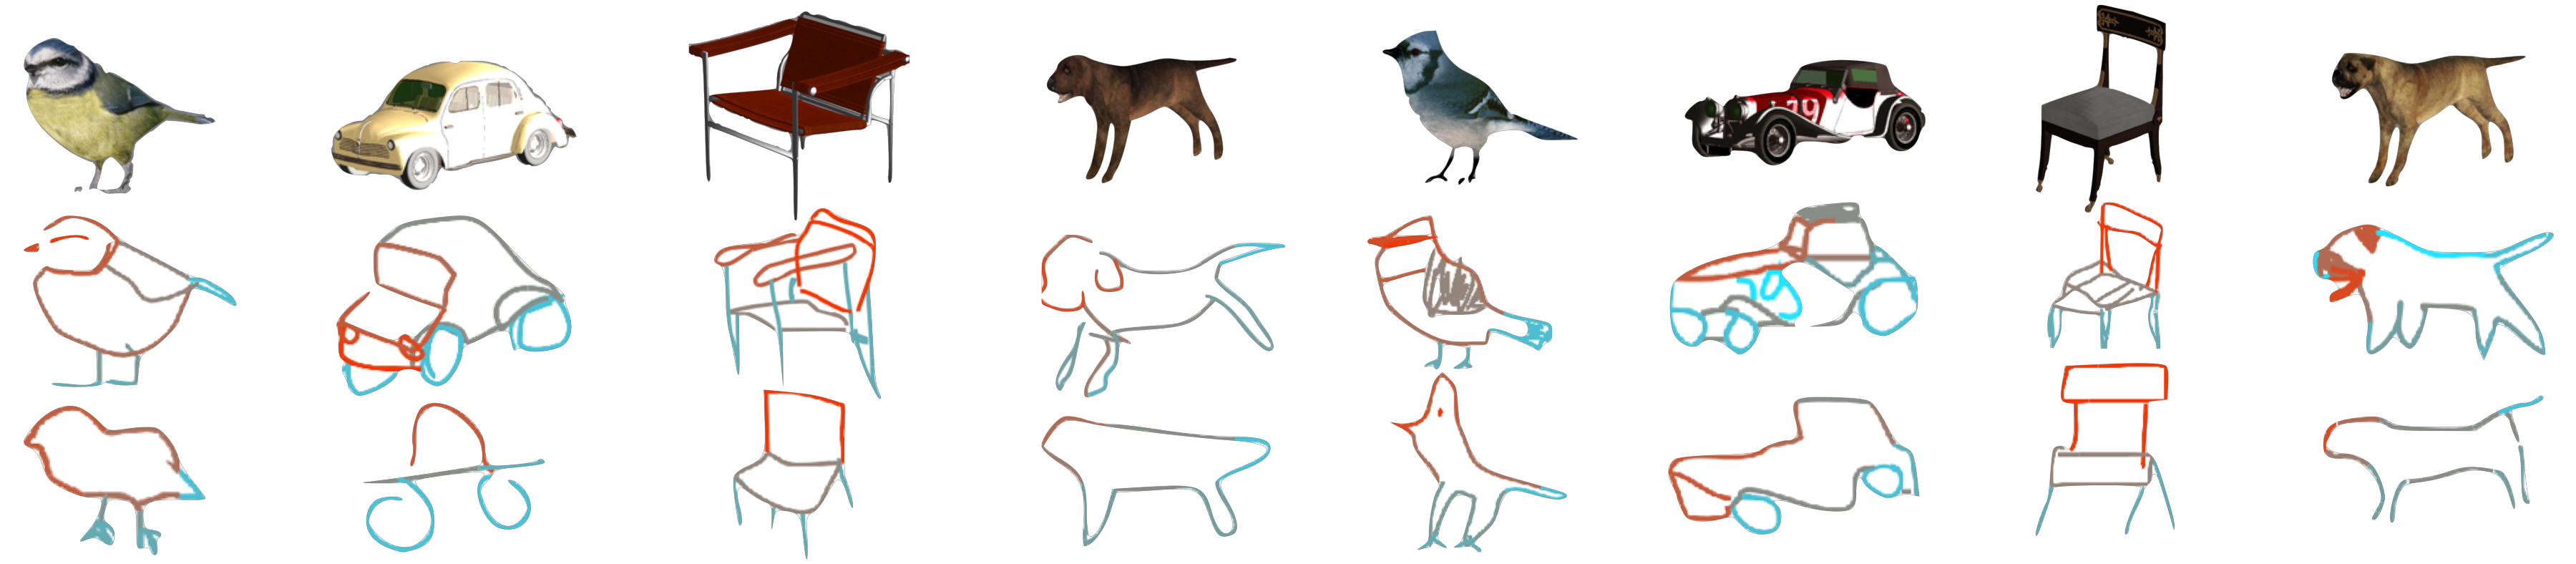
\includegraphics[width=0.92\textwidth]
    {figures/1_banner.pdf}
    \captionsetup{width=0.92\textwidth}
 \captionof{figure}{\footnotesize{Objects used in communication game with example drawings of each object, where stroke color indicates different parts.}}\bigskip} 
\makeatother

\maketitle 

\begin{abstract}
We effortlessly grasp the correspondence between a drawing of an object and that physical object in the world, even when the drawing is far from realistic. 
How are visual object concepts organized such that we can both recognize these abstract correspondences and also flexibly exploit them when communicating them to others in a drawing?
Here we consider the notion that the compositional nature of object concepts enables us to readily decompose both objects and drawings of objects into a common set of semantically meaningful parts.
To investigate this, we developed a web-based platform to densely annotate drawings of real-world objects with part information. 
Our dataset contained both detailed and sparser drawings produced in different communicative contexts.
We found that: (1) people are consistent in what they interpret individual strokes to represent. (2)Single strokes tend to correspond to single parts with (3)strokes representing the same part often being clustered in time. (4) Both sparse and detailed drawings of the same object emphasize similar part information but (5) detailed drawings of different objects are more distinct from one another than sparse drawings. 
Taken together, our results support the notion that people flexibly deploy their abstract understanding of the compositional part structure of objects to communicate relevant information about them in context. 
More broadly, they highlight the importance of structured knowledge for understanding how pictorial representations convey meaning. 





\textbf{Keywords:} 
sketch understanding; visual production; compositionality; objects and categories; perceptual organization
\end{abstract}

\section{Introduction}

%% revise so that the throughline is clearer: how does the human mind organize visual concepts such that they can be deployed so flexibly? answer: compositionality. what is a good way of probing compositionality? you could use discrimination tasks, but compositional tasks are much more direct. what is good about compositionality? it enables flexibility. how do you probe flexibility? compositional tasks across different contexts. 

When we open our eyes, we do not experience a meaningless array of photons --- instead, we parse the world into people, objects, and their relationships. 
The ability to represent semantically meaningful structure in our environment is a core aspect of human visual perception and cognition \cite{navon1977forest}. 
%As a testament to this ability, we effortlessly grasp the correspondence between a drawing of a particular object and that physical object in the world, even if the drawing is far from realistic \cite{eitz2012humans}. 
As a testament to this ability, we effortlessly grasp the correspondence between a particular physical object in the world and a drawing of the object.
Simple line drawings lack much of the rich visual information present in real-world objects including color, luminosity, and texture. This makes even well-made drawings far from realistic. 
How are visual object concepts organized such that they can robustly encode such abstract correspondences?
Here we explore the notion that perceiving these correspondences is supported by our ability to decompose both objects and drawings into a common set of semantically meaningful parts \cite{biederman1988surface}. 

Recent advances in computational neuroscience have provided an unprecedentedly clear view into the algorithms used by the brain to extract semantic information from raw visual inputs, including drawings, exemplified by modern deep learning approaches \cite{FanCommon2018,yamins2014performance}.
Nevertheless, a major gap remains in adapting such deep learning models to emulate the structure and flexibility of human semantic knowledge \cite{lake2017building}.
A promising approach to closing this gap may be to exploit the parsimony and interpretability of structured representations that reflect how visual concepts are organized in the mind \cite{battaglia2018relational}.

However, pursuit of this strategy relies upon a thorough empirical understanding of this conceptual organization and how people express this knowledge in natural behavior. 
We aim to contribute to this understanding by probing the expression of visual semantic knowledge in a naturalistic setting that exposes both its structure and flexibility: visual communication via drawing. 
This approach departs from the conventional strategy for inferring the organization of visual object concepts, which entails eliciting judgments with respect to a small number of experimenter-defined dimensions. 
By contrast, visual communication tasks permit participants to include any elements they consider relevant and combine these elements freely, yielding high-dimensional information about how people organize and deploy visual semantic knowledge under a natural task objective. 

% By interrogating the semantic structure of communicative drawings, the goal of this paper is to shed light on how the semantic organization of visual object concepts supports their flexible expression across contexts. 
% The goal of this paper is to interrogate the semantic structure of communicative drawings in order to shed light on how the semantic organization of visual object concepts 

While other works have addressed techniques for recognition of drawings \cite{ha2017neural,li2019photo}, through this paper we shed light on the correspondence between visual semantic knowledge and the procedure by which people robustly convey this knowledge in their drawings. That is, we focus on how semantic knowledge about object part-structure not only helps in decomposing objects during perception, but also on how this knowledge manifests in drawing production.
%The goal of this paper is to shed light on the correspondence between visual semantic knowledge and the procedure by which people robustly convey this knowledge in their drawings.
This paper advances recent work \cite{FanCommon2018} investigating how drawings convey semantic information in three ways: 
\textit{first}, we introduce a new dataset of drawings with dense part annotations, allowing an explicit focus on compositional part structure,
\textit{second}, we explore the link between this semantic structure and the temporal dynamics of drawing production,
and \textit{third}, we examine differences in how visual semantic knowledge is expressed between contexts. 

% \begin{figure}[htbp]
% \centering
% \includegraphics[width=0.48\textwidth]{figures/2_refgame_performance.pdf}
% \caption{(A) Drawings were collected in the context of a two-player drawing-based reference game in which one participant (sketcher) aimed to draw a target object so that the other participant (viewer) could distinguish it from three distractor objects. (B) In close contexts, the target and distractors all belonged to the same basic-level category; in far contexts, the target and distractors belonged to different basic-level categories. (C) sketchers used fewer strokes in the far condition, while producing drawings that were accurately recognized by the viewer in both conditions.}
% \label{refgame_performance}
% \end{figure}

\section{Methods}

We developed a web-based platform \cite{deLeeuw2015} to collect dense semantic annotations of the stroke elements in drawings of real-world objects (Fig. 1).
%These drawings were produced in different communicative contexts, including detailed and simpler drawings of each object.  

\subsection{Communicative drawing dataset}
We first obtained 1195 drawings of 32 real-world objects from a recent experimental dataset in which pairs of participants played an interactive drawing-based reference game \shortcite{fan2018modeling}. \footnote{All materials and data are available at \url{https://github.com/cogtoolslab/semantic_parts}.}
Object stimuli were photorealistic 3D renderings belonging to one of four basic-level categories (i.e., bird, car, chair, dog), each of which contained eight exemplars. %(Fig.~\ref{refgame_gallery}A).
On each trial of the experiment, participants were presented with a shared context containing four of these objects. 
One participant (the sketcher) was privately cued to draw a target object so that the other participant (the viewer) could pick it out from the set of distractors. % (Fig.~\ref{refgame_performance}A). 
Across trials, the similarity of the distractors to the target was manipulated, yielding two types of communicative contexts: \textit{close contexts}, in which all four objects belonged to the same basic-level category, and \textit{far contexts}, in which objects belonged to different basic-level categories. % (Fig.~\ref{refgame_performance}B). 
This context manipulation led sketchers to produce simpler drawings containing fewer strokes and less ink on far trials than on close trials, while still achieving high recognition accuracy in both types of context.% (Fig.~\ref{refgame_performance}C). %, Fig.~\ref{refgame_gallery}B\&C). 
 
% \begin{figure*}
% \centering
% 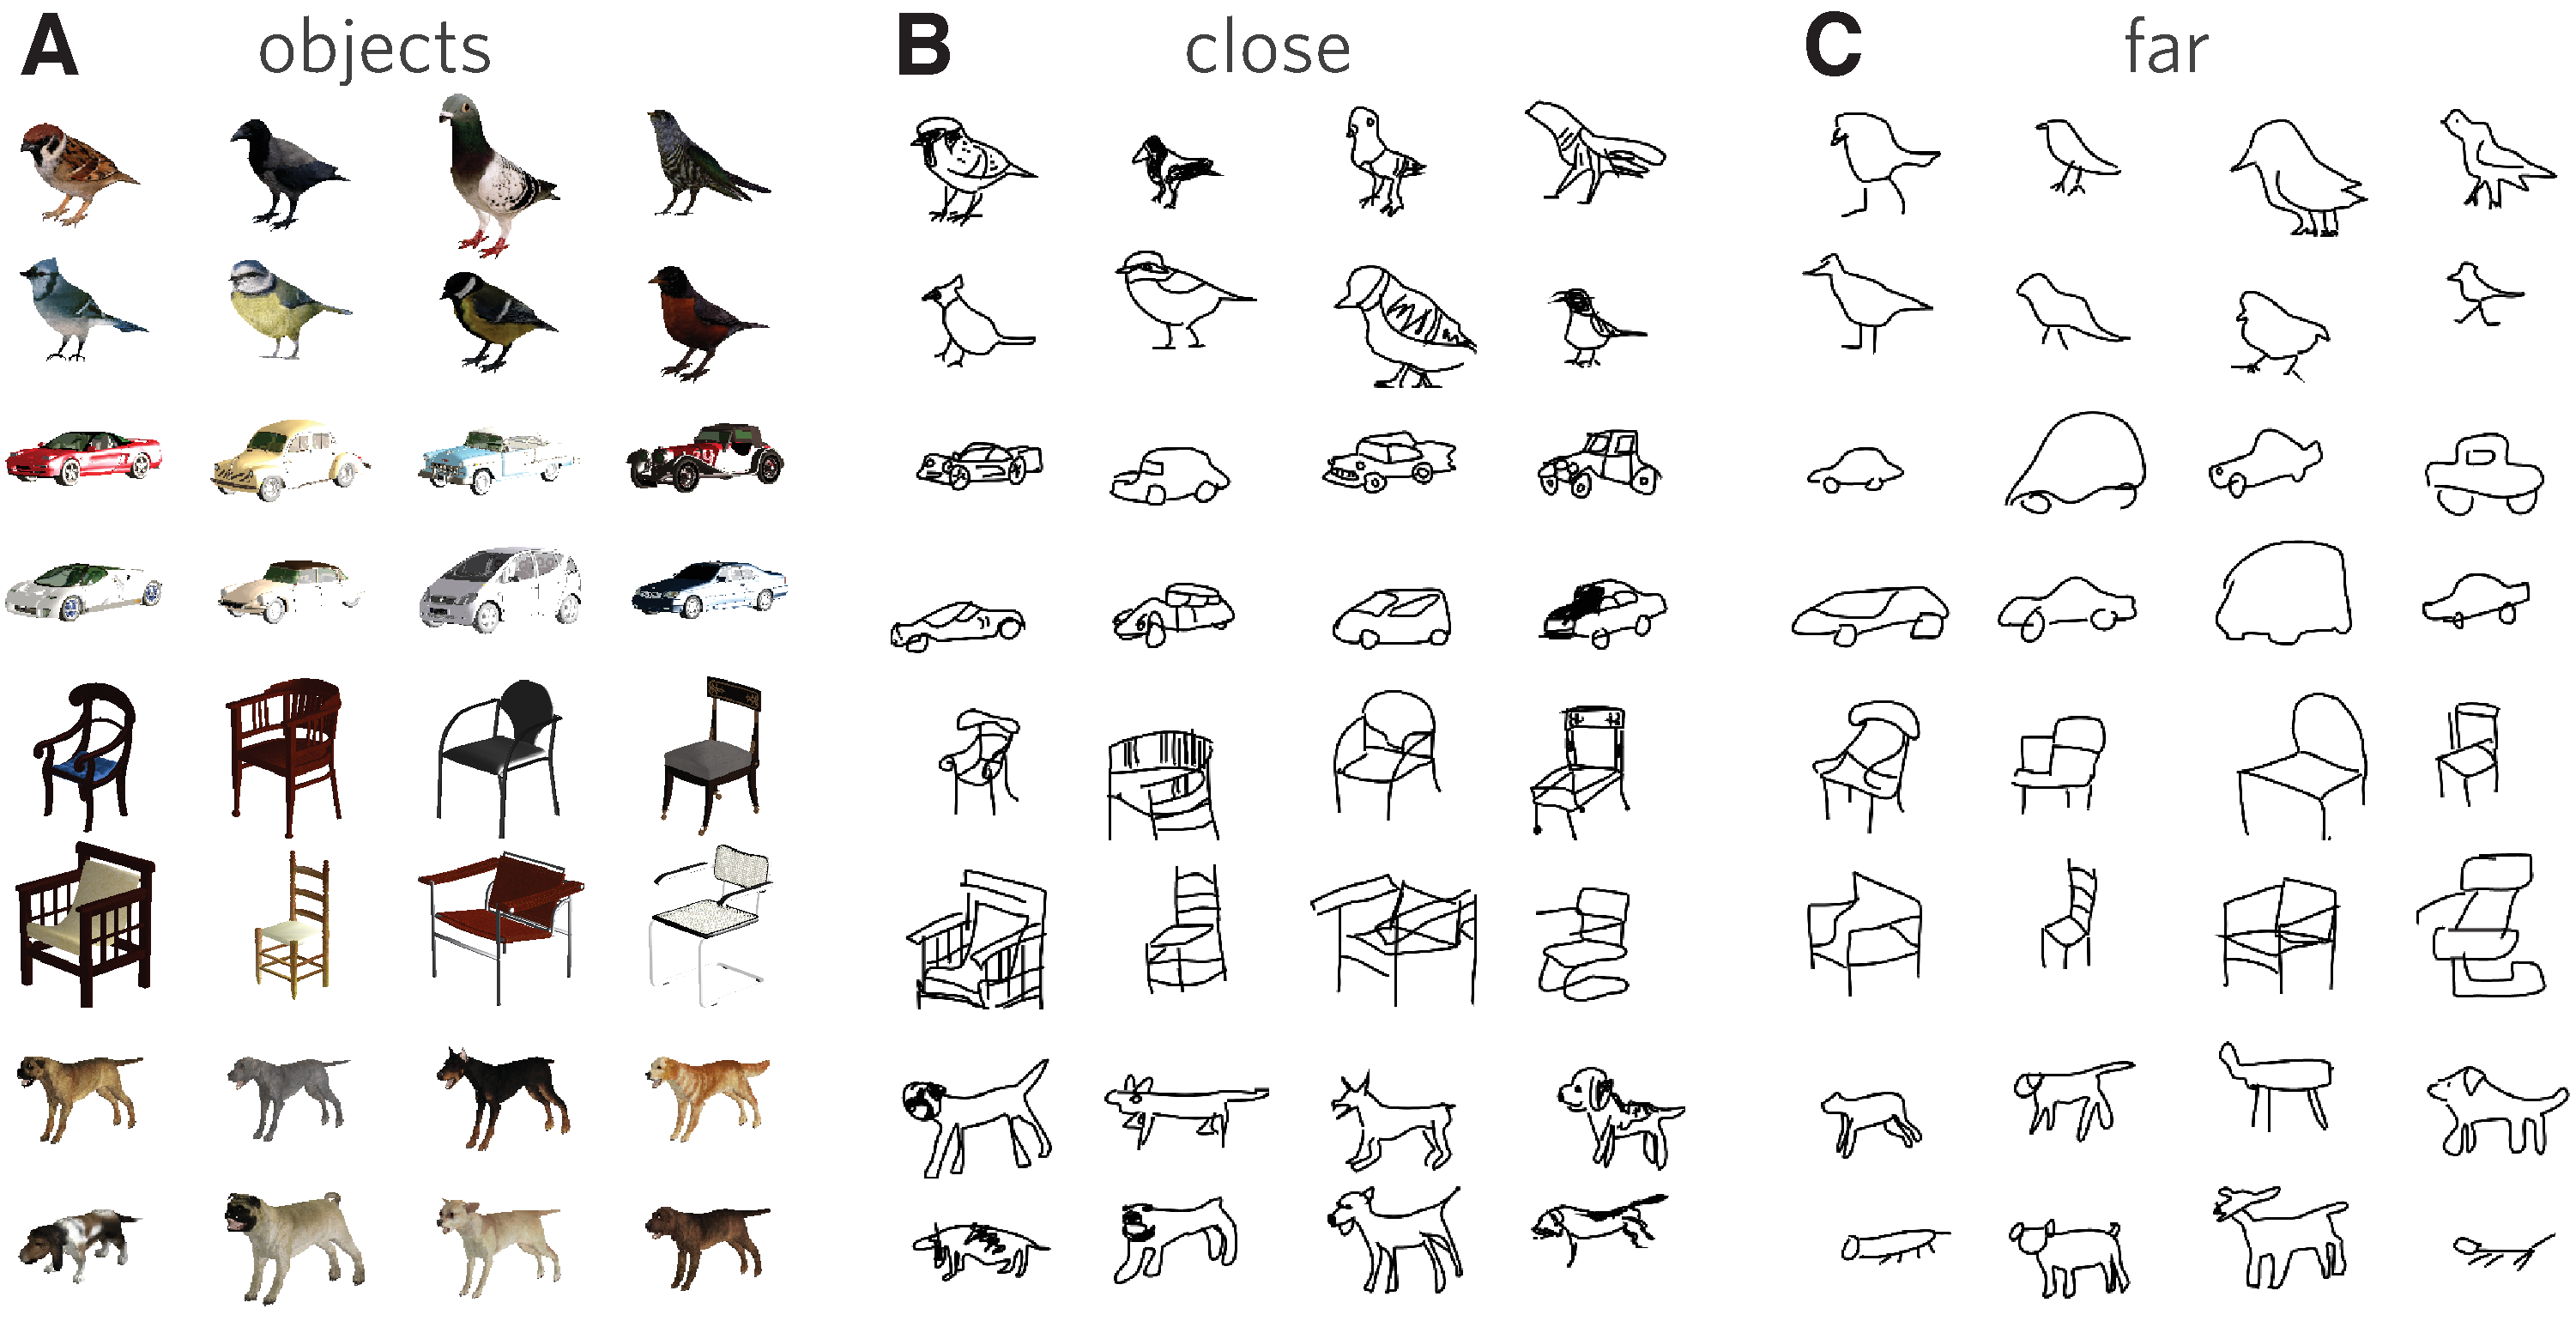
\includegraphics[width=0.95\textwidth]{figures/3_refgame_gallery.pdf}
% \caption{(A) Target objects. (B) Example object drawings produced in a close context. (C) Example drawings produced in a far context.}
% \label{refgame_gallery}
% \end{figure*}

Prior work analyzing the semantic properties of drawing data has used a raster image representation (e.g., \texttt{*.png}), an expedient format for applying modern convolutional neural network architectures \shortcite{FanCommon2018,sangkloy2016sketchy,yu2017sketch}. 
However, to investigate how semantic structure manifests during drawing production, it was critical to encode each drawing using a vector image format that preserves the inherently sequential and contour-based nature of drawing production (i.e., \texttt{*.svg}). 
Thus, each drawing in our dataset is represented as a sequence of individual strokes. A single stroke corresponds to a sketcher's decision to press the drawing tool to the canvas, make a mark, and raise the tool. 
Each stroke consists of a sequence of cubic Bezier curves, which we call \textit{splines}. 
This format provides a compact representation that preserves the sequence in which each element was produced.

\begin{figure}[htbp]
\centering
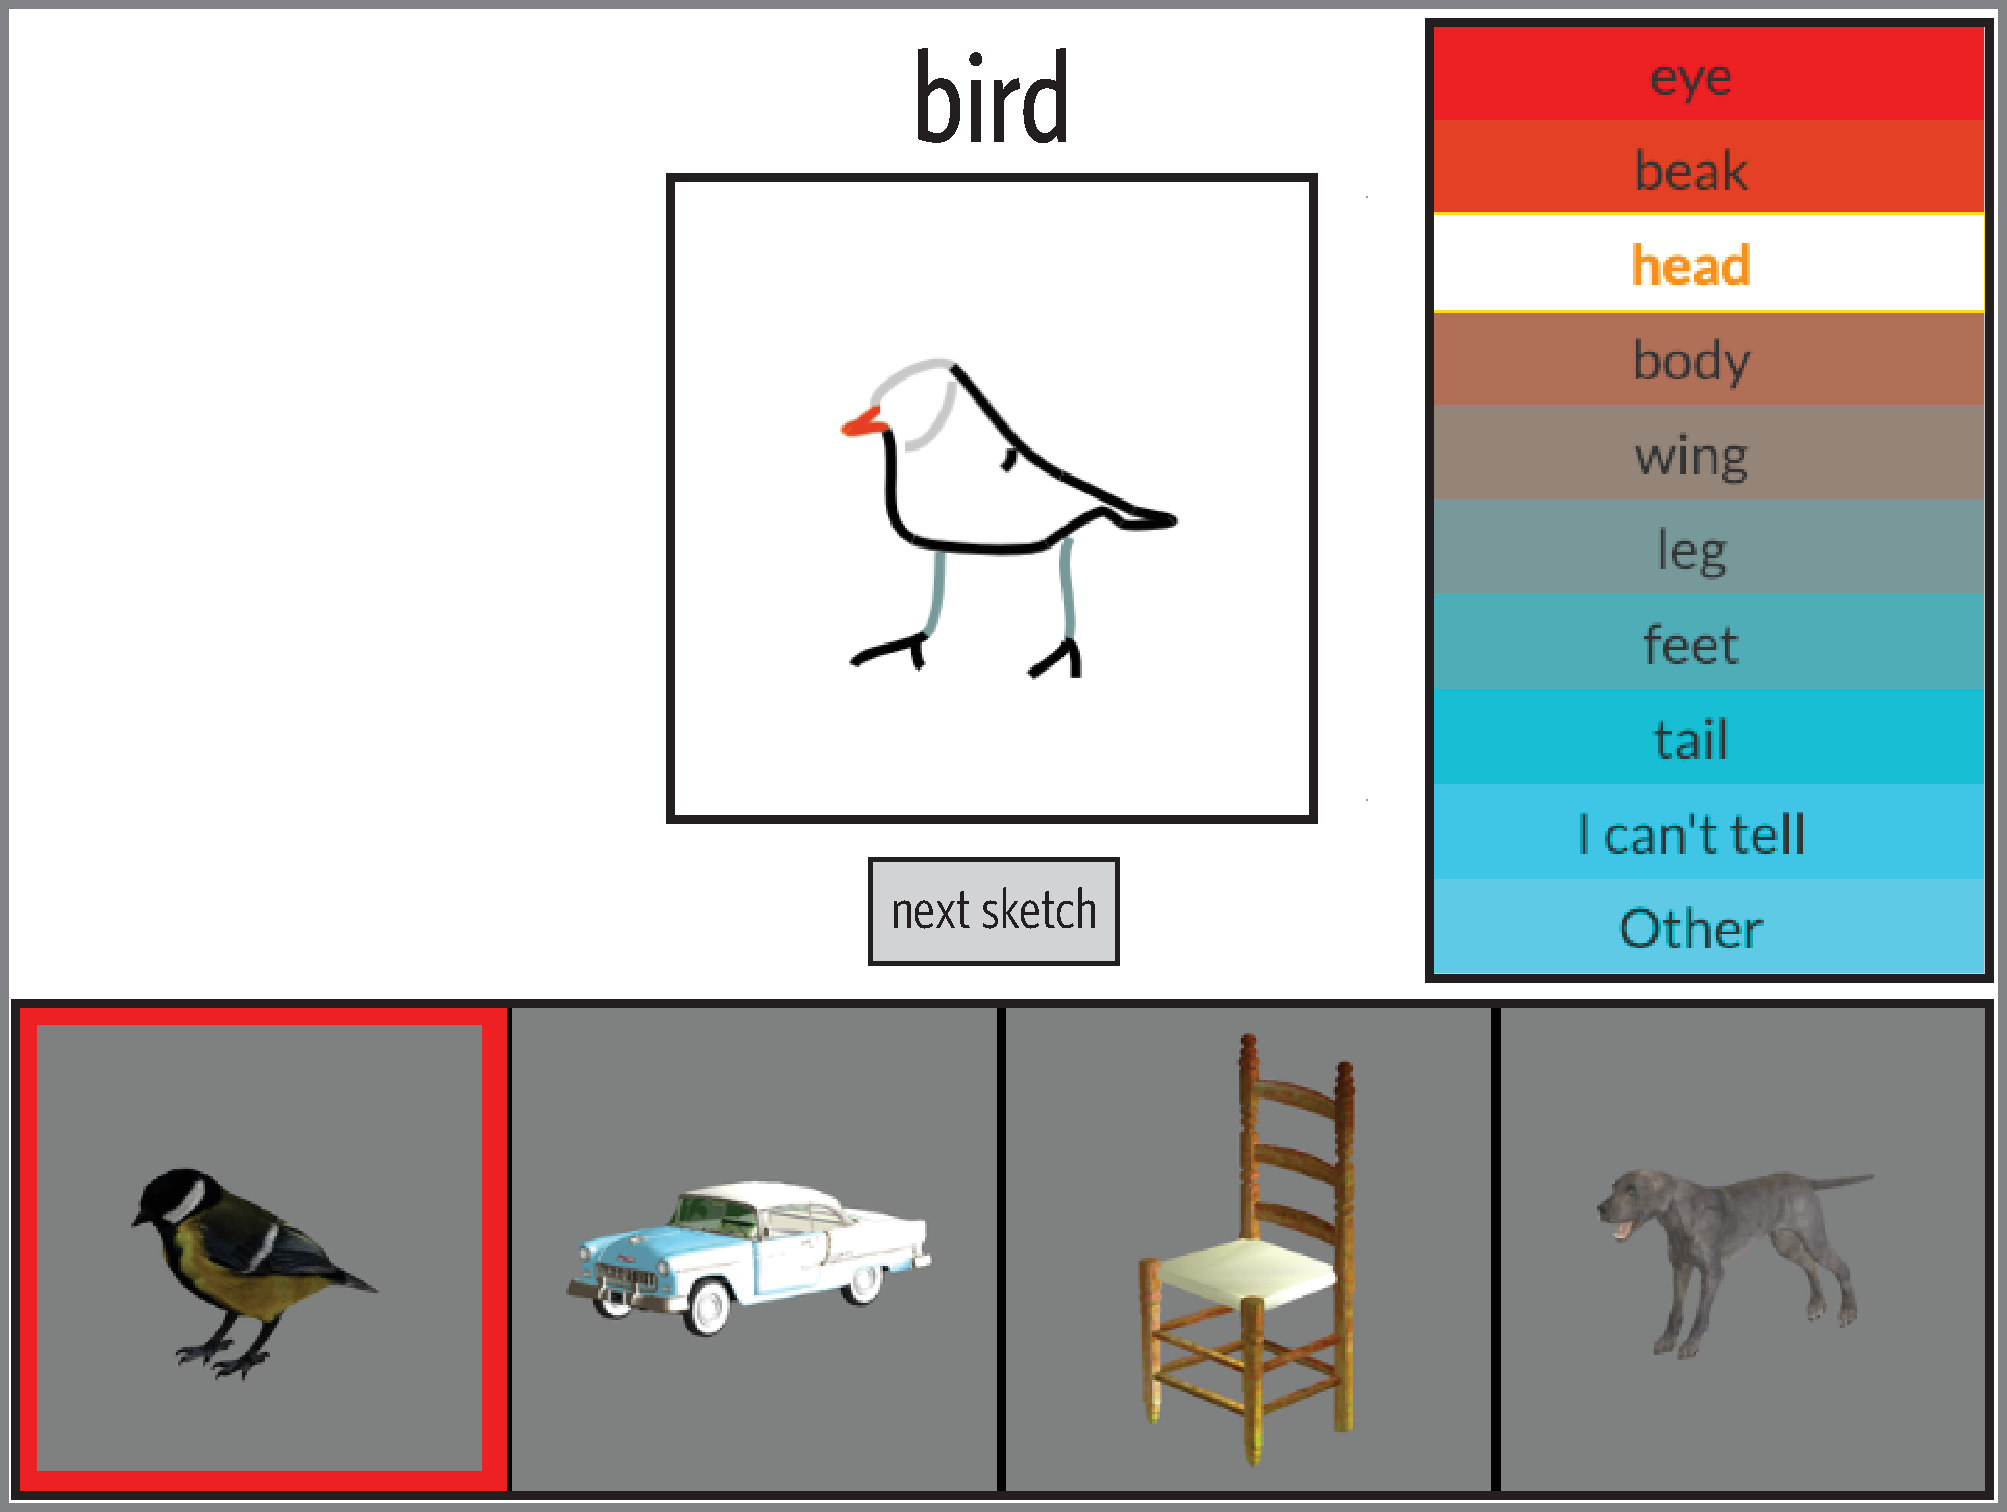
\includegraphics[width=0.47\textwidth]{figures/4_annotation_interface.pdf}
\caption{Annotation interface. Participants selected sub-stroke elements (splines) and tagged them with part labels.} %  from the menu The original communicative context in which the sketch was generated was also provided below the sketch.}% , with the target object highlighted in red and three distractors were displayed in an array below the sketch.}
\label{annotation_interface}
\vspace{-1em}
\end{figure}

\subsection{Semantic part annotation}

We then crowdsourced semantic annotations for every spline in every stroke of the drawings from this dataset. 
If splines were too short for annotators to feasibly annotate them, they were concatenated with a neighboring splines until the resulting spline was easily selectable with a mouse cursor.

\subsubsection{Participants}
326 participants were recruited via Amazon Mechanical Turk (AMT) and provided informed consent in accordance with the Stanford IRB. 
Participants were given a base compensation of \$0.35, plus \$0.002 for every spline they annotated and \$0.02 for every drawing they annotated completely. 

\subsubsection{Task procedure}
Each participant was presented with a sequence of 10 drawings that were randomly sampled from the communicative drawing dataset (Fig.~\ref{annotation_interface}). 
Their goal was to tag each spline with a label corresponding to the part it represented (e.g., seat, leg, back for a chair).  
To facilitate consistent tagging, participants were provided with a menu of common part labels that were associated with each basic-level category (Table \ref{tab:parts}).
Participants could also generate their own part label if they believed none of the common labels applied.
To give participants full information about the original communicative context, we showed the drawing with the same array of four objects that the original sketcher had viewed, with the target object highlighted in red. 

\subsubsection{Data preprocessing}
\begin{table}[b]
\vspace{-2em}
\begin{tabular}{ll}
\hline
\textbf{category} & \textbf{part labels} \\ \hline
bird & eye, beak, head, body, wing, leg, feet, tail \\ \hline
car & \begin{tabular}[c]{@{}l@{}}bumper, headlight, hood, windshield, \\ window, body, door, trunk, wheel\end{tabular} \\ \hline
chair & backrest, armrest, seat, leg \\ \hline
dog & eye, mouth, ear, head, neck, body, leg, paw, tail \\ \hline
\end{tabular}
\caption{Part labels provided to annotators.} % All user-generated labels were mapped to this set of labels.
\label{tab:parts}
\end{table}
To reduce bias due to missing data, we restricted our analyses to annotation trials in which the drawing was completely annotated (i.e., all splines were tagged).  %  when analyzing the relative emphasis that sketchers placed on different part information
Moreover, to ensure the reliability of our annotations, we only examined drawings that were annotated by three distinct participants. 
Our final preprocessing step was to incorporate manual part labels provided by participants (i.e. labels not in the menu).
Some of these labels were valid, but were synonymous with or subsumed by other more frequently occurring labels. 
For example, some strokes that represented subparts of the leg of a chair were labeled as `leg support', `foot', and `strut.'
In order to ensure that parts of drawings were segmented at a consistent level of granularity, we manually constructed a part dictionary to map these less-frequent part labels to one of the common part labels. 
After applying these preprocessing steps, our annotated dataset consisted of 864 drawings that had been annotated exactly three times each, using a set of 24 unique part labels. 

\section{Results}

\subsection{How well do viewers agree on what strokes mean?}

Before proceeding to use these annotations to examine how semantic information is conveyed during drawing production, we conducted a basic check of inter-annotator consistency. 
Specifically, we examined how often different annotators agreed on what each spline in a drawing represented.
We found that 95.6\% of all splines received the same label by at least two of the three annotators, and 67.8\% of all splines received the same label by all three annotators. 
This shows that the way viewers interpret which part each stroke represents is systematic, validating our general approach. 
Further, it suggests that sketchers may exploit this systematicity to produce strokes that they expect viewers to interpret consistently. 
In subsequent analyses, we collapsed over inter-annotator variation: we assigned the modal label to splines to which at least two annotators had given the same label; for the remaining 4.4\% of splines, we sampled one of the three labels provided.

\subsection{How do strokes correspond to parts of objects?}

When composing a recognizable drawing of a real-world object, how do sketchers decide what information to convey with each stroke? 
A natural possibility is that their actions closely correspond to the part structure of that object.
Concretely, we hypothesized that most strokes in our dataset would \emph{not} cross part boundaries: that all splines within a given stroke would be assigned the same part label. 
Conversely, because depictions of parts can be arbitrarily detailed, and some parts re-occur throughout an object (e.g., multiple legs on a bird, chair, or dog), we often expected to find more than one stroke per part  (Fig.~\ref{stroke_to_part}A).

\begin{figure}[htbp]
\centering
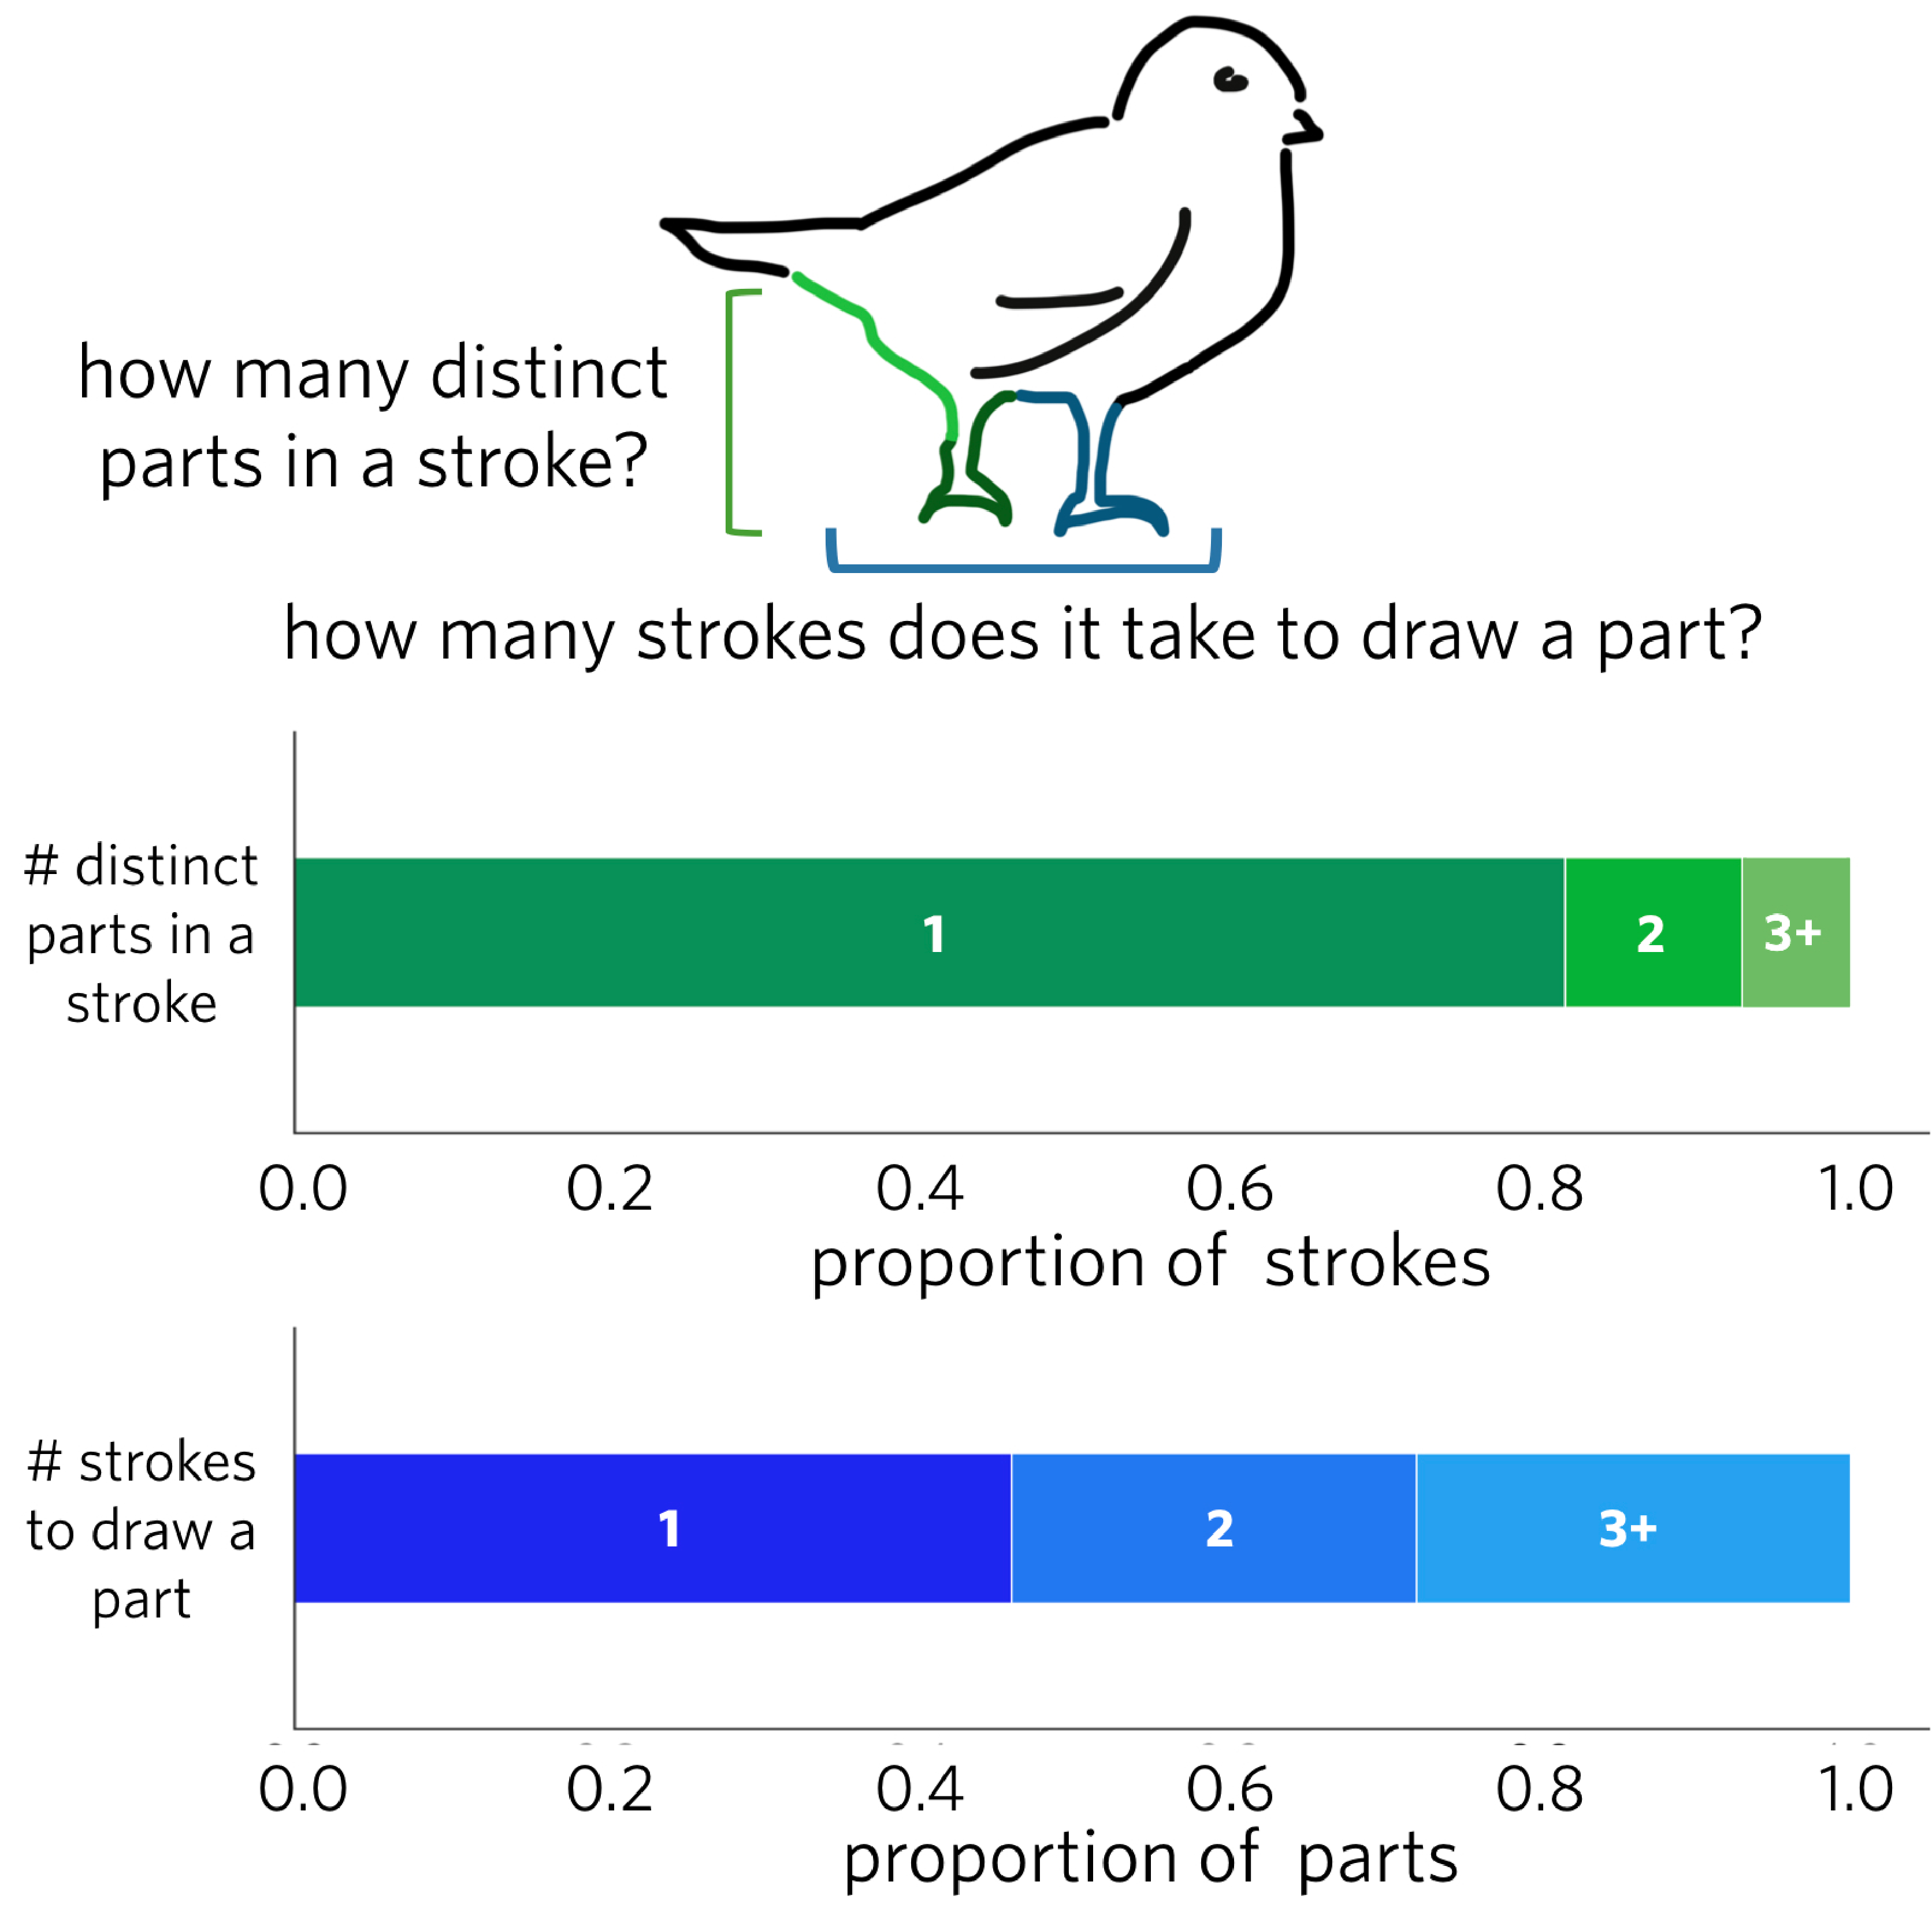
\includegraphics[width=0.45\textwidth]{figures/5_stroke_part_relationship.pdf}
\caption{(A) Analysis of correspondence between strokes and part labels: number of unique part labels assigned to different splines within the same stroke and number of different strokes used to draw each part. (B) Distribution over number of unique part labels within a stroke. (C) Distribution over number of strokes used to draw a part.}
\label{stroke_to_part}
\end{figure}

To evaluate the first hypothesis, we computed the number of unique part labels across all splines within each stroke. 
We found that for 81.6\% of the strokes in our dataset there was only one part label; the remaining 18.4\% of strokes were associated with two or more labels  (Fig.~\ref{stroke_to_part}B).

% Thus, most strokes represented exactly one part, but there were still a minority of cases where a single stroke spanned multiple parts (e.g., a single stroke connecting the head and body of a bird, or an armrest and leg of a chair). 
% These multi-part strokes were slightly more common in drawings produced in far contexts (19.4\%, CI: [17.9\%, 20.9\%]) than close contexts (17.6\%, CI: [16.1\%, 18.8\%]\footnote{95\% confidence intervals were estimated via stratified bootstrap resampling (N=1000 iterations) of drawings within each object-context combination.}). 
% This suggests that sketchers were somewhat more likely to use a single stroke to represent multiple spatially contiguous parts in a context that did not require them to produce a highly detailed drawing.

In other words, most strokes represented exactly one part, but in a minority of cases they spanned multiple parts (e.g., a single stroke connecting the head and body of a bird, or an armrest and leg of a chair). 
We were concerned, however, that these proportions were inflated by strokes with very few splines.\footnote{The modal number of splines per stroke (20\% of cases) was 1, but there was a long tail; the mean number was 2.6.}
To address this concern, we constructed a null model controlling for the number of splines.
Part labels were randomly sampled from the full list of parts in the drawing such that each spline was equally likely to represent any part regardless of the stroke it belonged to.
In simulations from this null model, only 55\% of strokes corresponded to a unique part while 45\% of strokes spanned multiple parts. 
Thus, individual strokes in our dataset were much more likely to correspond to a single part (i.e., not cross part boundaries) than would be expected under random assignment of part labels to splines.


To evaluate the second hypothesis, we computed the number of strokes that were used to represent each part of an object (Fig.~\ref{stroke_to_part}C). 
We found that 46.1\% of parts were depicted using exactly one stroke, 26.0\% using exactly two strokes, 11.3\% using exactly three strokes, and 16.6\% using four or more strokes. 
Thus, nearly half the time, a single action was sufficient to depict an entire object part. 
However, the remaining 53.9\% of the time, more than one stroke was required to depict an entire part, which would be expected for those parts that consisted of multiple disconnected subparts within an object (e.g., wheels of a car, paws of a dog).

% The proportion of parts requiring more than one stroke was slightly higher for close drawings (55.8\%, CI: [53.7\%, 58.6\%]) than far drawings (52.0\%, CI: [49.9\%, 54.6\%]), perhaps reflecting the tendency to include more detail per part to distinguish the target object from similar distractors. 
% Together, these findings suggest that the information people convey with each stroke systematically corresponds to the parts that objects contain. 


Together, these findings suggest that the information people convey with each stroke systematically corresponds to the parts that objects contain. 
We further hypothesized that these properties may vary between communicative contexts.
Indeed, strokes spanning multiple parts were slightly more common in drawings produced in far contexts (19.4\%, CI: [17.9\%, 20.9\%]) than close contexts (17.6\%, CI: [16.1\%, 18.8\%]\footnote{95\% confidence intervals were estimated via stratified bootstrap resampling (N=1000 iterations) of drawings within each object-context combination.}), suggesting that sketchers were somewhat more likely to use a single stroke to represent multiple contiguous parts in a context where a sparser drawing would be sufficient.
And the proportion of parts requiring more than one stroke was slightly higher for close drawings (55.8\%, CI: [53.7\%, 58.6\%]) than far drawings (52.0\%, CI: [49.9\%, 54.6\%]), suggesting that sketchers may have included more detail per part in close drawings to distinguish the target object from similar distractors. 


\subsection{Do strokes representing the same part tend to be produced in succession?}
\begin{figure}[t]
\centering
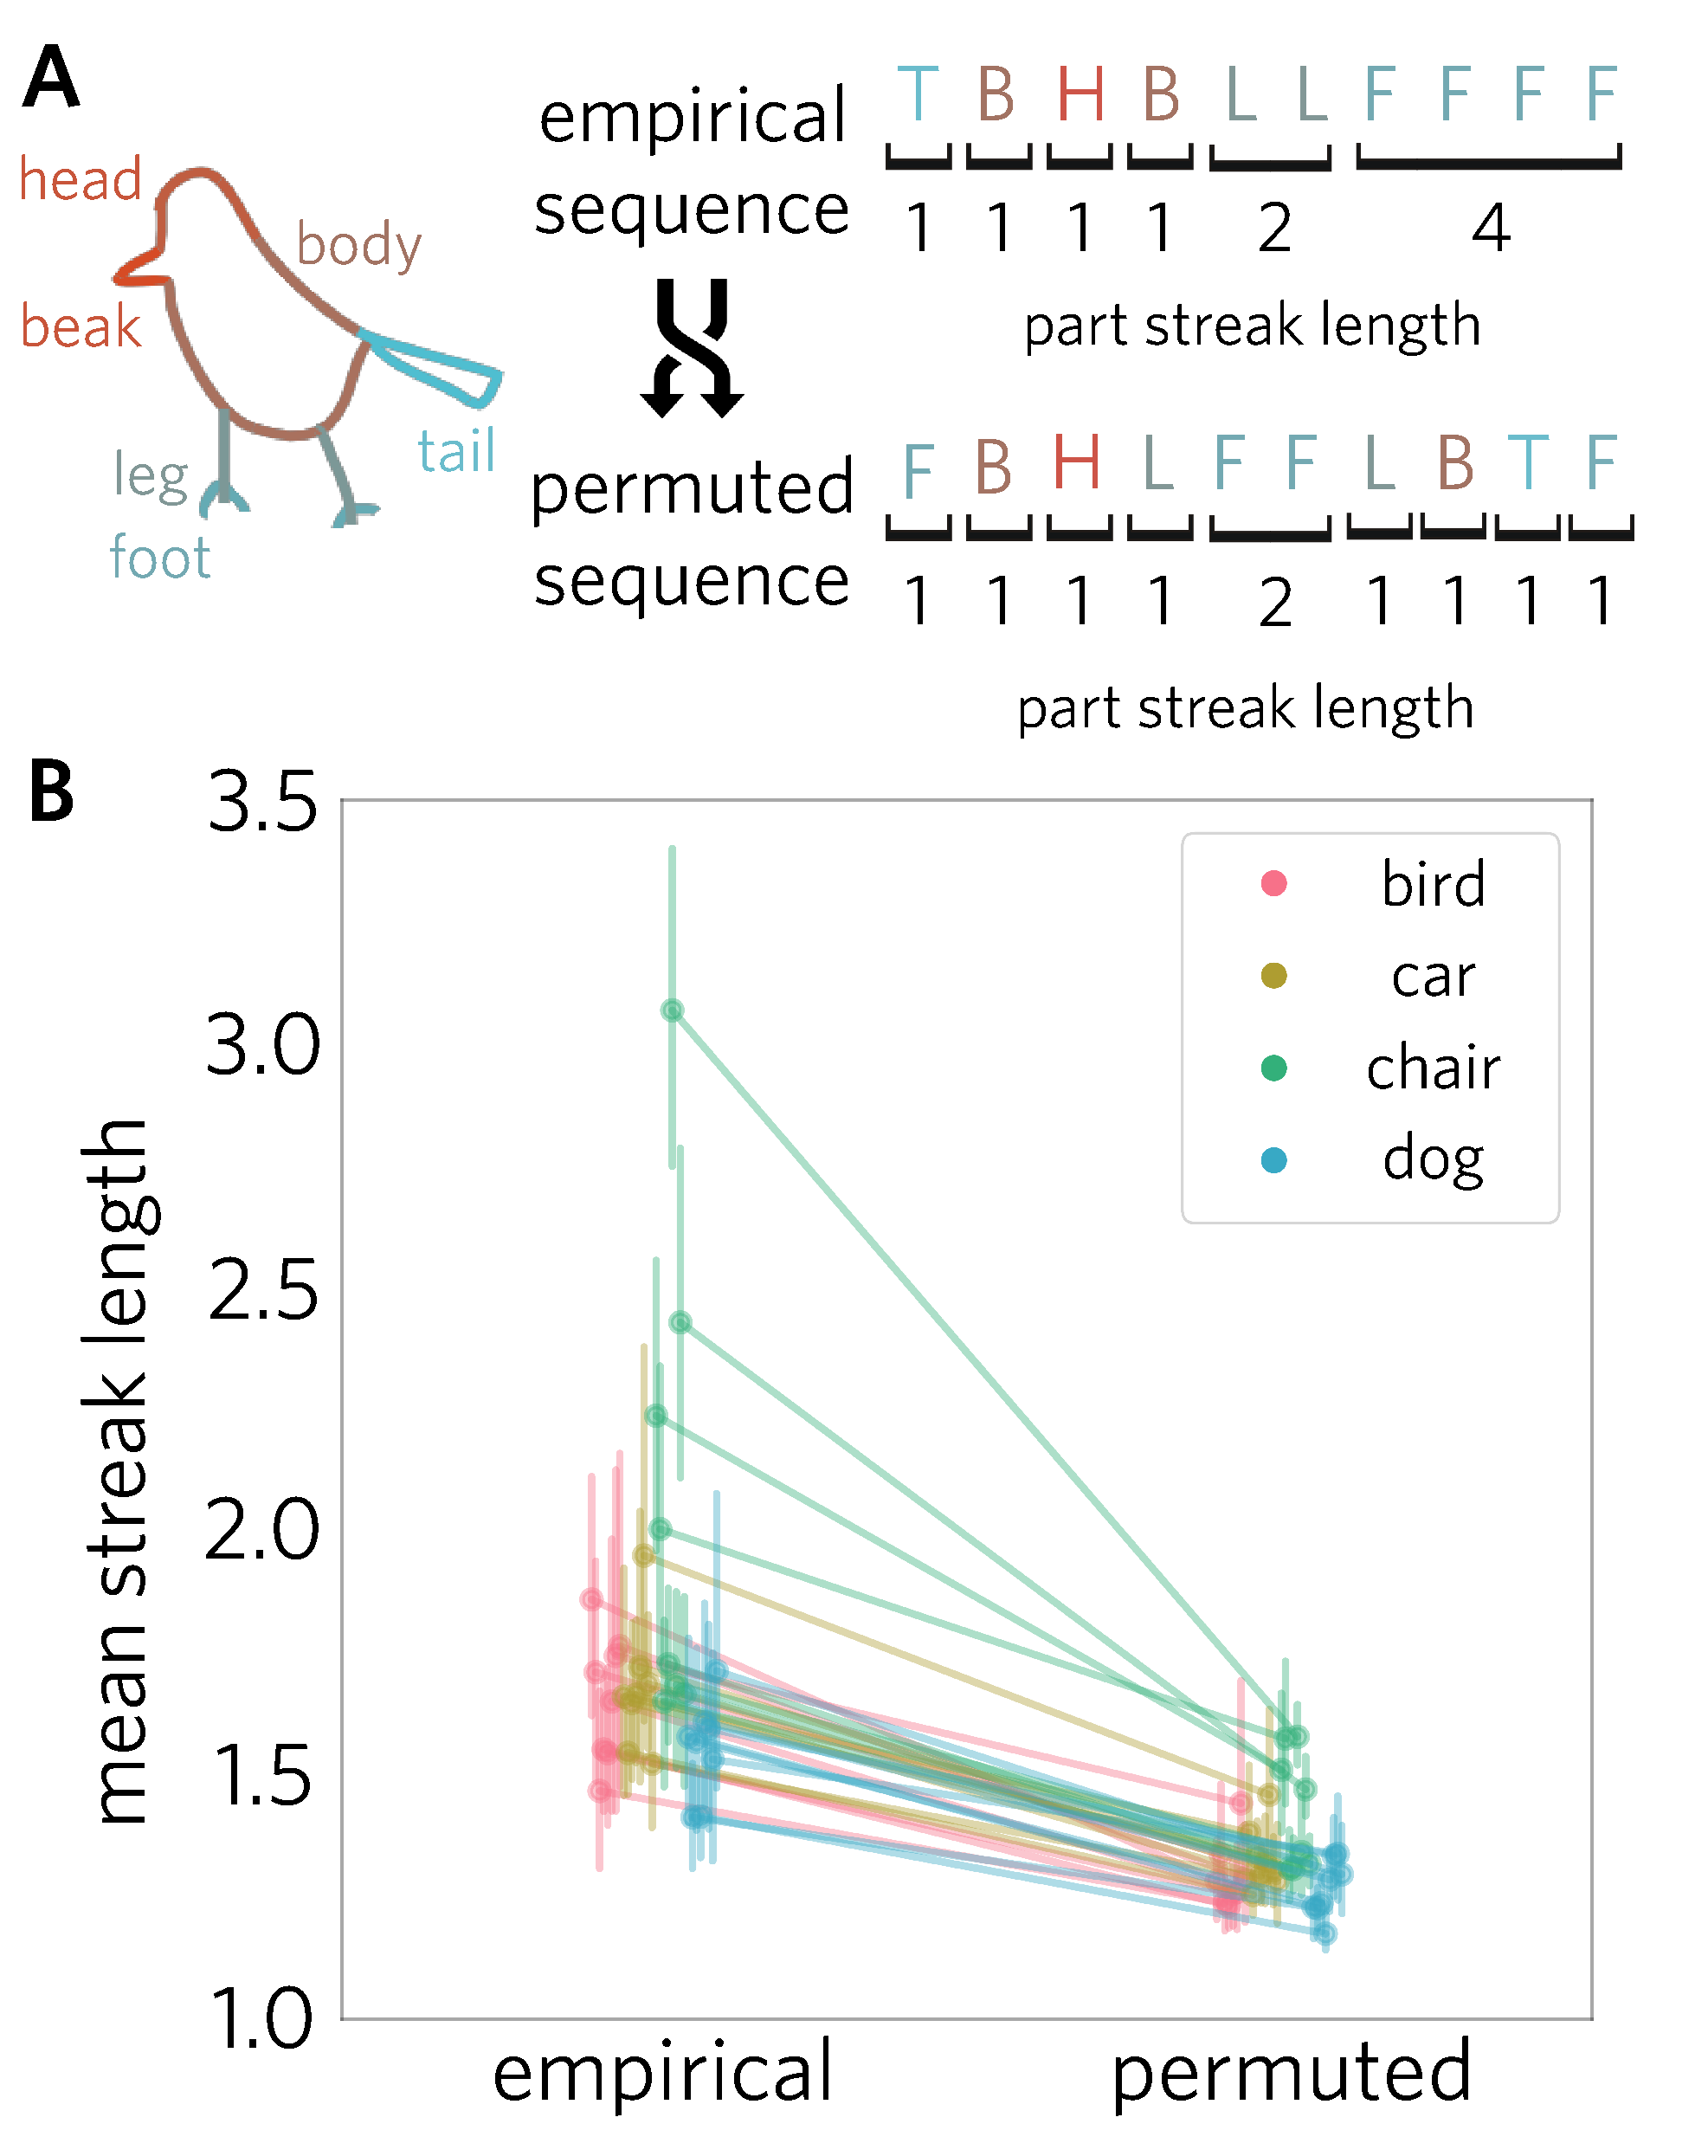
\includegraphics[width=0.5\textwidth]{figures/6_part_sequence.pdf}
\caption{(A) Analysis of sequence in which strokes depicting each part were drawn. (B) Comparison of mean length of streaks consisting of strokes that depict the same part with null distribution of permuted stroke sequences.}
\label{stroke_sequence_fig}
\end{figure}

In the previous section we discovered that slightly more than half of the parts in our dataset were depicted using multiple strokes. This result raised the question: to what extent are strokes depicting the same part drawn in succession, or interleaved among strokes corresponding to other parts?
In other words, how does the temporal sequence of stroke production relate to semantic part structure?

%To investigate this, we estimated the mean length of part streaks consisting of strokes depicting the same part, and compared this to the mean streak length for permuted stroke sequences. 
%We used mean streak length as a proxy for the prevalence of same-part strokes drawn in succession. 
% To investigate this, we computed for each sketch its part streak lengths — counts of the number of successive strokes depicting the same part drawn in succession — and compared the mean of these streak lengths to the mean streak length for permuted stroke sequences of the same sketch. 

To investigate this question, we estimated the mean length of streaks containing strokes depicting the same part.
First, we collapsed across the spline annotations examined in the previous section and represented each stroke by the modal part label assigned to its splines.
We represented each drawing as the sequence of these part labels, and defined \textit{part streak length} to be the number of consecutive strokes annotated with the same part label.\footnote{We excluded 78 out of the 864 drawings where this measure was not well-defined, i.e. sketches containing only one stroke or part label, or containing fewer than two strokes sharing the same part label.}
For example, in the drawing shown in Fig.~\ref{stroke_sequence_fig}A, two `leg' strokes were placed before moving on to the `foot', giving a streak of length 2.
Finally, we averaged these streak length values over every drawing in the dataset to obtain our statistic. 

To evaluate whether the empirical part sequences were more structured than expected if parts were drawn at random, we constructed a null model to serve as a baseline.
For this null model, we permuted the part sequence such that the number of instances of each part was preserved, but the temporal structure was disrupted (Fig.~\ref{stroke_sequence_fig}A).
We generated a null distribution of streak lengths for each drawing by repeating this permutation procedure 1000 times and measuring the mean streak length for each permutation.
Finally, we obtained a $z$-score for each drawing by computing where the empirical streak length fell in the permuted streak length distribution.
A drawing with a $z$-score near 0 had a streak length that was commonly obtained by placing strokes in a random order, while a drawing with a higher $z$-score is more structured than expected under the null.

We found that the empirical streak length was reliably higher for all objects than that of the permuted sequences (z-score: 2.07, CI: [1.90, 2.23]; Fig.~\ref{stroke_sequence_fig}B), and higher for the close drawings (z-score: 2.58; CI: [2.26, 2.90]) than far drawings (z-score: 1.56; CI: [1.38, 1.74]).
The lower streak length for far drawings is consistent with their lower stroke count overall---when only one or two strokes are used per part, there is a ceiling on the mean streak length. 
However, when sketchers do use multiple strokes to convey a single part (i.e., because there are multiple subparts, or to add more detail), they tend to draw these in succession before moving on to a different part.
These results suggest more broadly that the procedure by which people convey semantic information in drawings is organized by the part structure within objects.

\subsection{How is part information emphasized in different communicative contexts?}

Our findings so far bear on how the way people compose communicative drawings of objects reflects their semantic knowledge of the parts those objects are composed of.
A key consequence of such semantically organized part knowledge is that it naturally supports flexible expression across different communicative contexts. 
For example, when communicating about a chair in a far context containing objects from other basic-level categories, sketchers may include only the essential information to indicate the presence of certain parts (e.g., armrests) that distinguish it at the category level. 
On the other hand, when communicating about that same chair in a close context containing other, perceptually similar chairs, sketchers may emphasize aspects of parts that distinguish it at the object level (e.g., the curvature of the armrests), by applying more strokes and/or more ink in each stroke.

We hypothesized that sketchers emphasize part information to preserve relevant distinctions in context. 
To explore this possibility, we asked the following questions: 
(1) How similarly is object-specific part information emphasized in close and far contexts? 
% (2) To the extent close and far drawings of the same object emphasize part information differently, does this reflect large differences in emphasis on a few parts, or small differences in emphasis across many parts? 
(2) How do differences in how part information is emphasized across contexts affect the discriminability of drawings?

To investigate these questions, we represented each drawing by a \textit{part-feature vector} that combined information about: (a) how many strokes and (b) how much total ink was expended on each part of that object. 
In order to represent all drawings in our dataset using a common feature representation, we combined part labels across categories, yielding a set of 24 unique part labels to which any stroke could be assigned. 
Each part-feature vector thus consisted of 48 elements: 24 of these represented the number of strokes allocated to each part, and the remaining 24 represented the total arc length of all strokes allocated to each part. 
Before further analysis, we z-scored values within each feature dimension in order to map stroke-count and arc-length measurements to the same unit-variance scale. 
Because our primary goal was to understand differences between objects and contexts, we then collapsed across drawings within each object-context combination, yielding 64 average part-feature vectors (i.e., 32 objects x 2 context conditions). 

\vspace*{4px}

\subsubsection{Similar part information emphasized across different communicative contexts}

In order to investigate to what extent similar object-specific part information is emphasized in different communicative contexts, we computed the matrix of Pearson correlations between part-feature vectors. 
Formally, this entailed computing: $R_{ij} =  \nicefrac{cov(\vec{r}_{i}, \vec{r}_{j})}{\sqrt{var(\vec{r}_{i}) \cdot var(\vec{r}_{j})}}$, where $\vec{r}_{i}$ and $\vec{r}_{j}$ are the mean part-feature vectors for the $i$th and $j$th object-context combinations, respectively.

While close and far drawings of an object differed in their overall amount of detail, we hypothesized that they would still emphasize part information in similar ways.
Specifically, insofar as similar object-specific part information is emphasized in both close and far drawings of the same object, we predicted higher correlations between close and far part-feature vectors for the \textit{same} object than for close and far part-feature vectors of \textit{different} objects. 
Consistent with this, we found strong correlations between the feature vectors for close and far drawings of the same object ($r = 0.740$,  CI: [0.726, 0.753]), which were significantly stronger than close and far drawings of \emph{different} objects ($r = 0.653$, CI: [0.646, 0.659]).
These results show that close and far drawings of the same object exhibit similar \emph{patterns} of emphasis across different parts, and this similarity exceeded that expected due to merely being members of the same basic-level category (Fig.~\ref{part_emphasis}B). 

\vspace*{4px}

% \subsubsection{Greater emphasis on a few parts when producing detailed drawings}

% Although the patterns of emphasis on different parts were similar between close and far drawings, close drawings expressed more part information overall.
% To what extent do close drawings accomplish this by placing a lot more emphasis on a few parts, or placing a little extra emphasis on many parts?
% To address this question, we first calculated the vector difference between the close and far part-feature vectors for each object.
% % To provide a geometric intuition, each difference vector represents the direction and distance to move in this 48-dimensional feature space to get from the centroid of the far drawings of an object to the centroid of its close drawings. 
% If close drawings place a lot more emphasis on a few parts, this difference vector will be sparse, containing a few large non-zero values and many zero values. 
% On the other hand, if close drawings tend to place a little extra emphasis on many parts, this difference vector will not be non-sparse, containing many similar non-zero values and few zero values. 
% We used the following metric to compute the sparsity of each difference vector:
% $\texttt{s}= \nicefrac{(\sqrt{k} - \frac{\norm{v}_1}{\norm{v}_2})}{(\sqrt{k}-1)}$, where $k=48$ (the dimensionality of the vector), $v$ is the difference vector, $\norm{v}_1$ is the L1-norm and $\norm{v}_2$ is the L2-norm. 
% Here, $s=1$ for maximally sparse vectors (i.e., single non-zero value) $s=0$ for minimally sparse vectors (i.e., all values identical and non-zero).
% We found that difference vectors were moderately sparse ($s=0.675$, 95\% CI: [0.653, 0.686]), suggesting that close drawings place more emphasis on a few different parts relative to far drawings, but not to the same extent for all parts (Fig.~\ref{part_emphasis}C).

\subsubsection{Detailed drawings are more distinct from each other than sparser drawings}


While the above findings showed that close and far drawings of the same object exhibit similar patterns of emphasis on different parts, close drawings contain greater emphasis on these parts overall than far drawings (i.e., contained more and longer strokes). 
How were these additional strokes being spent? 


We hypothesized that the additional part information provided in close drawings was being distributed across parts in different ways for different objects, thereby making them more distinguishable from one another in feature space.
% This would have the consequence of increasing the feature distance between close drawings, 
To evaluate this possibility, we computed the mean correlation between the part-feature vectors of close drawings of objects in a given category and compared this value with the mean correlation between far drawings of exactly the same objects. 
We found that close drawings were less similar to one another than far drawings were (close similarity: $r = 0.67$, CI: [0.65,69]; far similarity: $r = 0.73$, CI: [0.72,0.75]), suggesting that sketchers discern which parts are most diagnostic of the target object among highly similar distractors, and emphasize these parts accordingly (Fig.~\ref{part_emphasis}C).
This was particularly apparent when we visualized the spatial layout of part-feature vectors: whereas far drawings were clustered closer together and near the origin, close drawings were spread further apart from other members of the same category and further from the origin (Fig.~\ref{part_emphasis}A).
Observing these contextual differences is all the more remarkable given that this feature representation captures only the \textit{amount} of emphasis allocated to each part during drawing production, ignoring their visual properties. 


\begin{figure}[ht]
\centering
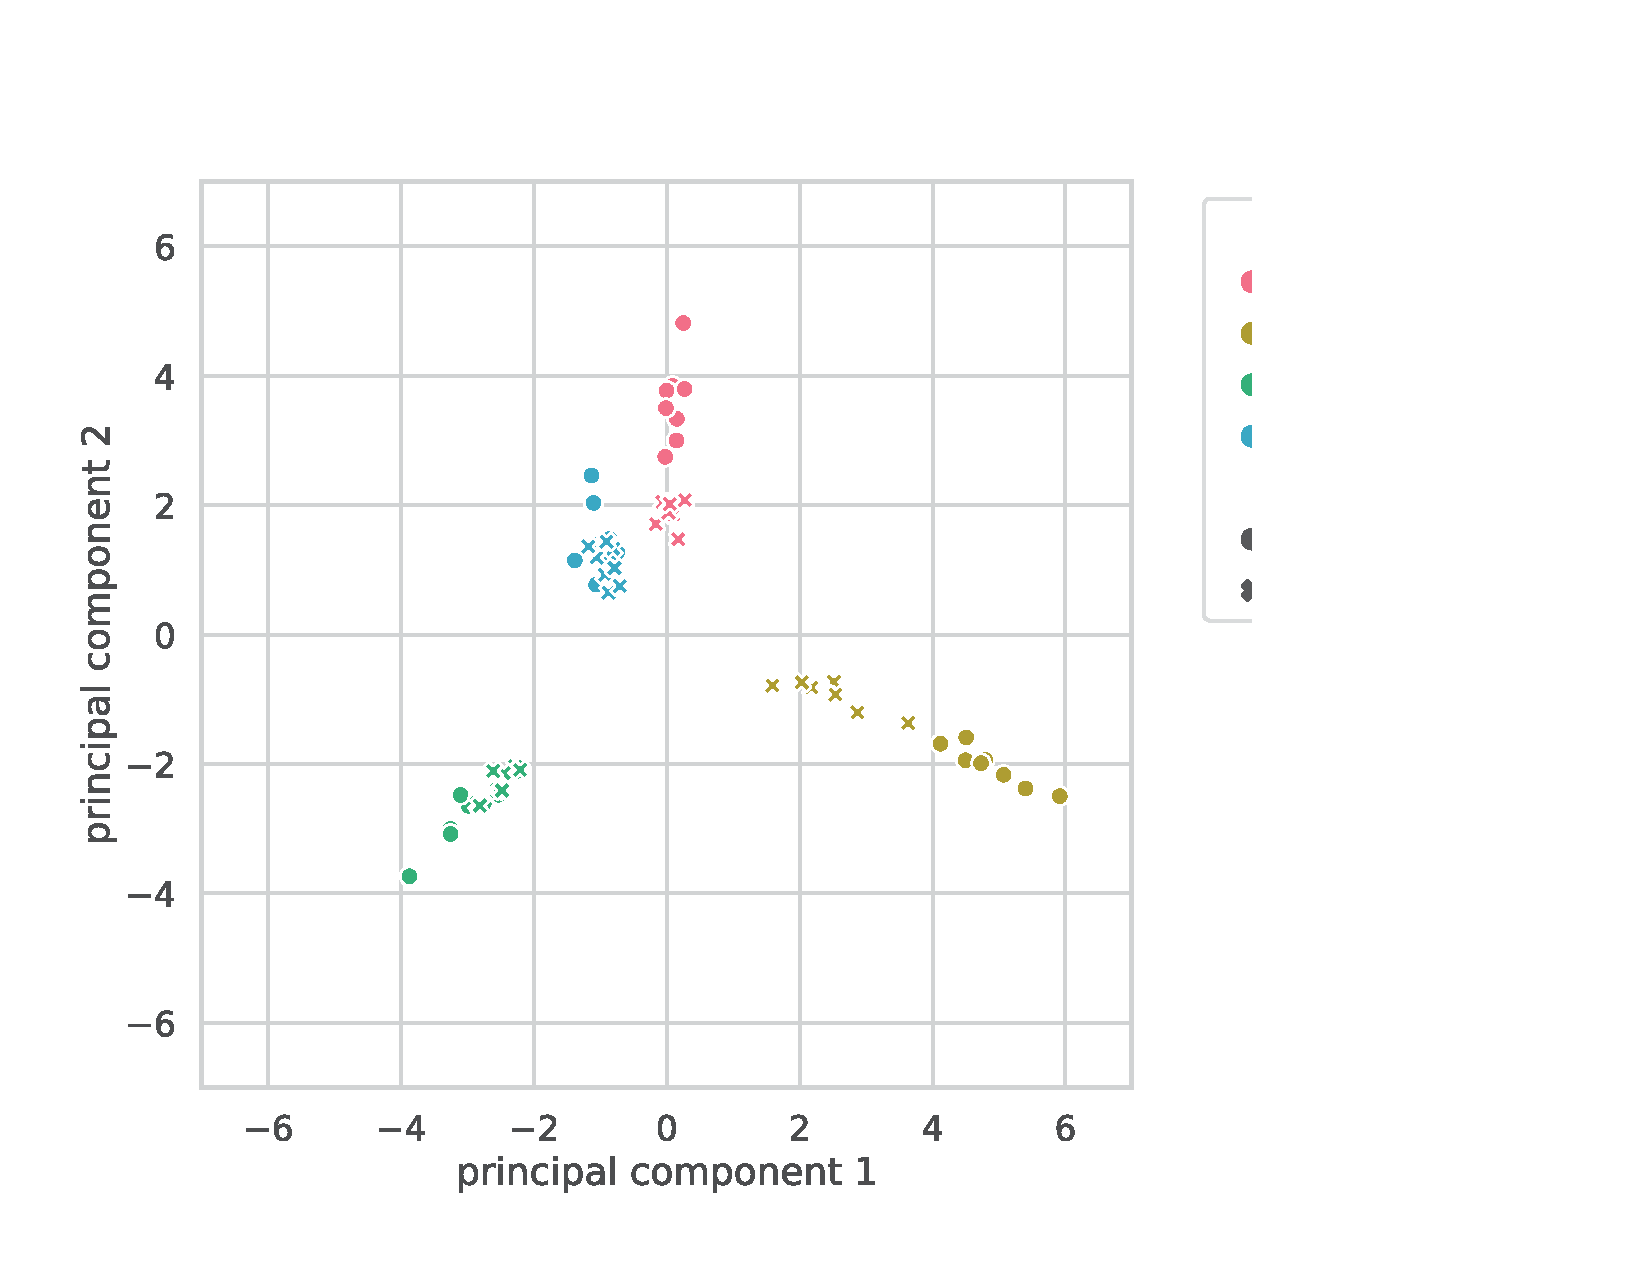
\includegraphics[width=0.38\textwidth]{figures/7_part_emphasis.pdf}
\caption{(A) Visualization of spatial layout of mean part-feature vectors for each object-context combination, projected onto the top two principal components. (B) Comparison of feature similarity between close and far drawings of the same object, relative to close and far drawings of different objects within a category. (C) Comparison of feature similarity between far drawings of objects within a category, relative to close drawings. *** \textit{p}$<0.001.$}
\label{part_emphasis}
\end{figure}

\section{Discussion}

In this paper, we explored how the way people compose communicative drawings of objects reflects their semantic knowledge about what objects are composed of. 
To accomplish this, we developed a novel web-based platform to collect dense semantic annotations of the stroke elements in drawings of real-world objects that were produced in different communicative contexts. 
Overall, we found that: (1) people are highly consistent in how they interpret what individual strokes represent; (2) single strokes tend to correspond to single parts; (3) strokes representing the same part tend to be clustered in time; and (4) detailed and sparse drawings of the same object emphasized similar part information, although (5) detailed drawings of different objects tend to be more distinct from one another than simpler ones. 
Taken together, our results support the notion that people deploy their abstract understanding of the compositional part structure of objects in order to select actions to communicate relevant information about them in context.  

While we believe that extending our approach to larger drawing datasets of many different object-categories with a large variety of parts would help establish the robustness of our findings, our results are nonetheless an important first step in establishing a meaningful relationship between drawing production and semantic knowledge. 

These findings are resonant with classic and recent work that has argued for the importance of compositionality in human perception and cognition in general \cite{biederman1987recognition, battaglia2018relational,lake2017building}, and for visual production in particular \cite{lake2015human}. 
However, unlike prior work which focused on the production of abstract symbols \cite{lake2015human}, we consider the challenge of how people transform perceptually grounded representations of real-world objects into procedures for producing figurative drawings that communicate not only what they see and know about them, but also what is relevant. 

Our work is also related to recent progress in the development of computational models of drawing production \cite{ha2017neural,li2019photo}. 
While results from these efforts have been galvanizing, the development of principled metrics by which to rigorously evaluate how well they emulate human drawing behavior has not kept pace. 
By interrogating in detail how humans encode semantic information into their drawings, and flexibly adjust their production behavior in different contexts, this paper presents a first step towards such a set of behavioral metrics. 
Having such metrics is important because they would enhance our ability to distinguish between generative models, and thereby help advance further model development. 
In summary, we establish the importance of semantic part-based knowledge in drawing production, highlighting the importance of compositionality in cognition, and the potential for using our findings to devise new metrics to sevaluate models of drawing production. \kushin{This last sentence sounds repetitive to me when I read it, but maybe it's good to have it as a summary statement of sorts?}

In future work, we plan to extend our analysis of how different part information is expressed in drawings beyond simple effort cost measures (i.e., number of strokes, amount of ink) to encompass content and style information (e.g., the shape of a bird's wing, caricaturization of a chair's armrest). 
We expect that augmenting current vision models with a combination of the requisite semantic part knowledge and the ability to discern perceptual properties of these parts, such as style, will allow us to build models that parse drawings in a more human-like way.

%We expect that this will entail augmenting current vision models with the requisite compositional semantic part knowledge to parse drawings in a more human-like way. 
More broadly, achieving this synthesis will lead to both more robust artificial intelligence and a deeper understanding of human cognition and behavior. 

% %%%%%%%%%%%%%%%%% informal sketch of discussion %%%%%%%%%%%%%%%%%%%%%%%

% %% summary of main findings parallel to abstract: I recommend using the same language from the abstract where we enumerate the main findings, preserving the sequence in which those findings appear in the paper. The wording can be slightly different but it should be immediately recognizable as parallel to the earlier summary of findings.

% %% this paper is about sketch *production*
% %% what is distinct about the current approach is its focus on linking fine-grained semantic knowledge about real objects to dynamics of drawing production. this is distinct from lake omniglot paper, which did not consider real objects. this is distinct from most approaches to studying fine-grained semantic knowledge, b/c of focus on production. or sketches, which has focused on holistic image properties. 

% % sketch-rnn: object production but not compositional
% % lakeomniglot: compositional production but not objects
% % sketchrecognets: objects but not production and not compositional
% % here: we consider compositional production of objects

% %% future work should use data like ours as benchmarks to validate models of visual production (e.g., sketch-rnn and that new contour drawing paper: https://arxiv.org/pdf/1901.00542.pdf) -- 
% % with data like these: compositionality-in-drawings becomes  an important target for modern theories/models of human visual cognition, which should be able to display this kind of human-like robustness, flexibility, expressivity.
% %% do next-gen models emphasize part information in a similar way? do they accomplish shifts in abstraction in a similar way to the way humans do? 

% %% Taken together, our results support the notion that people deploy their abstract understanding of the compositional part structure of objects in order to select actions to communicate relevant information about them in context. More broadly, they highlight the importance of structured knowledge for understanding how pictorial representations convey meaning.

% %%%%%%%%%%%%%%%%%%%%%%%%%%%%%%%%%%%%%%%%





% %%%%%%%%%%%%%%%%%%%%%%%%%%%%%%%%%%%%%%%%


% We show here that people are highly consistent in what parts they interpret drawings' constituent strokes as representing. 
% When the sequential strokes that a sketcher produces to create a drawing are coded in terms of these parts, we see that there is a prevalent one-to-one correspondence between individual strokes and parts. 
% We also observe that it is common for strokes representing the same part to be drawn in succession.
% We take these results to support the idea that people's semantic knowledge of objects helps guide their decisions on what to depict through their strokes and how to organize these strokes in time.
% The structure of completed drawings reflect this semantic part knowledge, even when drawings are produced in different contexts to varying degrees of detail. Detailed drawings of objects distinguish themselves from their sparser counterparts by preferentially expressing object-specific parts through their constituent strokes. However, both detailed and sparse drawings of objects preserve elements that help distinguish them from sketches of other objects.

% By focusing on the number and length of strokes as well as their sequence, we are able to study the correspondence between observable semantic structure in sketches and the decisions sketchers make to express this structure graphically.
% And these decisions reveal to us that people are able to decompose an abstract object into part-categories and reconstruct it in a flexibly structured manner during graphical production. The flexibility is in modulating which parts to express to what degree, given the contextual needs of communication.
% Our findings support the idea of compositionality in abstract visual conceptions of objects and categories.\cite{lake2015human, biederman1987recognition} 
% Such a form of representation is powerful for categorizing novel objects, discerning object identity through sparse or noisy channels, \kushin{too vague maybe?} and expressing concepts cheaply, as we see in the sparse drawings in our reference game dataset. 
% Compositional organization of semantically meaningful components in varied relationships to each other allows for an adaptive perceptual system that is nevertheless sensitive to the prevalence of commonly occurring elements in our environment \cite{Goldstone2003}. 

% Taken as a whole, these results show that drawings reveal people's conceptual knowledge of objects through how components of the object are expressed through strokes. We show that by considering the number of strokes and amount of effort expended in producing each stroke we are able to account for how drawings are able to flexibly convey information across different communicative contexts. Future work will look to investigate the properties of the parts that these strokes represent, i.e., the quality of the content they express over just the quantity and organization of semantically meaningful parts. This would allow us to understand how the perceptual properties of objects and parts influence this semantic decomposition

% % \kushin{need to tighten this paragraph to have a narrative throughline}


 
 \section{Acknowledgments}
KM was supported by the Department of Cognitive Science at Vassar College through its Humanities in Cognitive Science program.
RXDH was supported by the National Science Foundation Graduate Research Fellowship (DGE-114747). 

%\section{References}

\bibliography{semantic_parts}
\bibliographystyle{apacite}
%\setlength{\bibleftmargin}{.125in}
%\setlength{\bibindent}{-\bibleftmargin}






\end{document}
